\section{Methods} \label{Methods}

\subsection{Exploratory analyses}
    Principal Component Analysis (PCA) was performed on the arrayCGH dataset to explore its structure and investigate the potential separability of subgroups. PCA was conducted with scaling applied, together with analysis of principal components and their explained variance, using the 'stats' package (version 3.6.3) for the statistical programming language R (version 3.6.3, \citealp{R2020})
    Various clustering methods were investigated, including K-medoids and cosine distance (k = 3, pam() function from R package 'cluster', version 2.1.0), hierarchical clustering (Euclidean distance, average-linkage, dist() and hclust() functions from R package 'stats').

\subsection{Cross-validation}
    A nested cross-validation scheme with a stratified 10-fold outer loop containing a stratified 10-fold inner loop was implemented to validate the model performance together with that of feature selection and hyperparameter tuning. Training and test datasets of the outer and inner loops were divided 70\% / 30\%, respectively, using createDataPartition() from R package 'caret' (version 6.0-86, \citealp{Kuhn2008}). The inner loop was used for feature selection with Pearson's chi-squared test or Boruta (\citealp{Kursa2010}) and hyperparameter tuning (see below), the specific features and hyperparameters of the highest accuracy inner loop model were subsequently used in the outer loop. For each neural network, K-nearest neighbors (KNN) or Nearest Shrunken Centroids (NSC) classification model combined with either feature selection method, the final model was selected based on the highest accuracy score of 10 outer loop iterations.

    \begin{figure}[]%figure1
        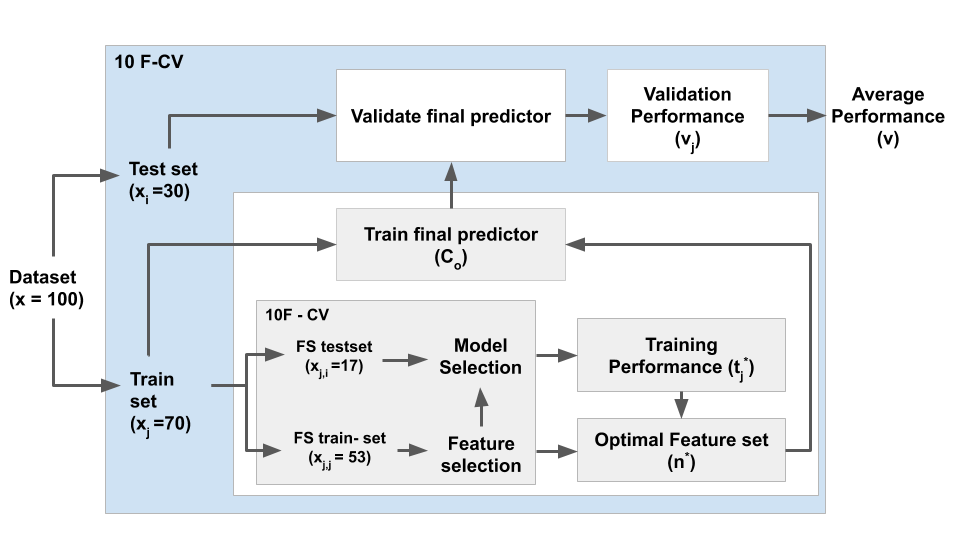
\includegraphics[scale=0.28]{CATS assignment/final-paper/cabios-template/images/figure_1.png}
        \caption{Train-validation schematic depicted in a simplified format. The input is the breast cancer aCGH dataset and output is the final predictor model with average performance.}\label{fig:01}
    \end{figure}

\subsection{Feature selection}
    Pearson's chi-squared test was used as statistical feature selection method and Boruta (\citealp{Kursa2010}) was used as wrapper feature selection method.
    Chi-squared tests were conducted on all 2,834 genomic regions individually using the function chisq.test() of the R package 'stats'. Contingency tables were constructed of clinical subgroups versus chromosomal aberration values. A Bonferroni-correction was applied to a significance threshold of 0.05 to correct for multiple testing, the corrected threshold being $2834 * 0.05$. The effect of various significance thresholds on the number of selected features and the training accuracy was investigated in order to select the most adequate threshold. The nested cross-validation scheme (previously described) was used with a 1-fold outer loop and 10-fold inner loop to investigate the effect of different thresholds (0.05, 0.01, 0.001) with additional Bonferroni-correction on the training set accuracy as well as the validation set accuracy and number of selected features.
    Boruta was implemented with the function Boruta() from the R package 'Boruta' (version 6.0.0). Random forest models were trained on the original dataset together with 'shadow' versions of randomized features to asses the importance of individual features for model performance. Feature importances were determined by two-sided hypothesis tests of equality of Z-scores between original and shadow version, where features were considered important if their Z-score was higher than that of the shadow versions  (\citealp{Kursa2010,kursa2014}). Undecided or "tentative" features were corrected for with the TentativeRoughFix() function using default parameters.

\subsection{Classification models and hyperparameter tuning}
    Neural network, KNN and NSC classification models were developed to classify breast cancer subgroup status for samples based on chromosomal aberration values (previously described). All models were implemented with the function train() from the R package 'caret'.
    Neural network models were trained with the value 'nnet' for the 'method' parameter of the function train(), which employed a single hidden layer feed-forward network (SLFN). Hyperparameters were tuned by passing combinations of 'decay' (ranging 5 to 7) and 'size' (0.1, 0.01, 0.001) to the 'tuneGrid' parameter of train().
    KNN models were trained with the value 'knn' for the 'method' parameter of the function train(). Hyperparameters were tuned by passing values of 'k' (ranging 1 to 10) to the 'tuneGrid' parameter of train().
    NSC models were trained with the value 'pam' for the 'method' parameter of the function train(). Hyperparameters were tuned by passing values of 'threshold' (ranging 1 to 8) to the 'tuneGrid' parameter of train().

\subsection{Hierarchical clustering}
    Hierarchical clustering of feature subsets from specific classification models was conducted using the function heatmaply() from the R package 'heatmaply' (version 1.1.0) using average-linkage (UPGMA) clustering by passing 'average' to the parameter 'clust\_method'.
    
\subsection{Permutation analysis}
    Permutations of the best-performing neural network model training set were conducted to assess the likelihood of obtaining that accuracy score by chance under similar conditions. Samples were first divided in 70\% training and 30\% test data that was representative for clinical subgroup distributions (createDataPartition() function of 'caret'). Second, feature sets of identical size to the best-performing model (38 features) were randomly sampled with replacement from the full feature space ($n = 2,834$). Third, neural networks were trained with the train() function from 'caret' using permuted training sets and identical hyperparameters to the best performing model (size = 5, decay = 0.01, MaxNWts = $10 * (size * (n.o. features + 2) + size + 1)$, maxit = 100). Fourth, accuracy scores were obtained from comparing model predictions with the actual subgroup status of test samples. In total 1,000 permutations were conducted, the Pvalue for the best-performing model's accuracy was calculated as the number of observations with equal or higher accuracy than the original (0.895).